\documentclass[main.tex]{subfiles}
\begin{document}

\chapter{Results}\label{ch:results}

\section{Data Sets}
The data presented in this chapter was collected during one hour of parallel measurements with both the analog and the digital setup. A total of 4.3 million pulses from the NE213 detector were recorded by the analog setup, while the digitizer only saw 2.2 million pulses after the selection criteria explained in the previous chapter were applied. This large difference in count rates is because the digital setup was configured to transfer each event individually. Furthermore the software WaveDump does not have a method for estimating livetime, so instead a livetime will be estimated by comparing with the analog setup.

Thresholds of 25.0 mV and 94.6 mV were applied to the YAP and the NE213 detector respectively in the analog setup, while the digital setup applied thresholds of 9.8 mV and 48.8 mV on the YAP and the NE213 detector. Having such a low threshold on the YAP was found to decrease the signal to noise ratio in the time of flight spectrum, so a higher threshold of 24.4\si{\milli\volt} was applied in software.
\begin{table}[bh]
\begin{tabular}{|l|l|l|l|l|}
\hline
Setup   & YAP threshold(mV) & NE213 threshold(mV) & NE213 events ($\text{10}^\text{6}$) & Livetime \\ \hline
Analog  & 25.0              & 94.6                & 4.3      & 44\%             \\ \hline
Digital & 9.8/24.4*			& 48.8                & 2.2      & **             \\ \hline
\end{tabular}
\caption[Overview table of the two data sets.]{Overview table of the two data sets. *The higher threshold was enforced offline (see text for details). **The digital setup does not have a method for determining livetime}
\label{tab:settings}
\end{table}

\section{Analog Setup}

\subsection{Neutron Tagging}
Figure \ref{fig:tof_a} shows the time of flight spectrum recorded by the analog setup. The neutron and gamma ray peaks marked with arrows. In addition to these two peaks there is an approximately flat background. This background represent uncorrelated particles triggering start and stop, which is why negative time of flight values appear.
\begin{figure}[ht]
    \centering
        \includegraphics{AnalogResults/tof.pdf}
        \caption[Time of flight spectrum, analog setup.]{The time of flight spectrum. The x-axis denotes the time of flight from source to NE213 detector. The neutron and gamma peaks have been indicated with arrows. The coincidences highlighted in red have been converted to neutron kinetic energies and are shown in the upper right insert.}
    \label{fig:tof_a}
\end{figure}

The gamma ray peak has been shifted to be centered at \SI{3.5}{ns}, but it is not entirely narrow. Since the gamma rays travel at the speed of light one might expect a much narrower gamma peak. This is primarily due to the time resolution of the detector as well as attenuation in the cables, which might affect pulse shape and thus rise time. This will in turn make the constant fraction discriminator less effective causing some loss in the time resolution. Furthermore, the final  digitization by the TDCs may cause some loss of resolution. Differences in flight path between gammas hitting the center of the NE213 and those that hit near the edge will be less than 1 cm, so this will not give rise to a substantial time spread. 

The neutron peak has faster neutrons at lower time of flight values and slower neutrons at higher time of flight values. Since the distance from source to detector is known it is possible to convert the neutron time of flight into kinetic energy. A range of 1.5-\SI{7}{\MeV} was converted to a time interval of 29-\SI{62}{\ns}. The coincidences falling in this time interval have been highlighted in red and the corresponding energies are shown in figure \ref{fig:tof_a}, where higher flight times map to lower energies.

Comparing to the spectrum obtained by Scherzinger\cite{ScherzingerPhd} and shown in \ref{fig:scherzinger} a couple of differences stand out. Scherzingers spectrum had peaks around \SI{3}{\MeV} and \SI{4.8}{\MeV}, whereas this spectrum only has a peak at \SI{4.5}{\MeV}. This spectrum on the other hand appears to have a peak near \SI{3.8}{\MeV} and one between 4 and \SI{5}{\MeV}. The absence of the \SI{3}{\MeV} peak may indicate that a higher threshold was applied when acquiring this data set. At low energies the counts in figure \ref{fig:tof_a} increases. This is simply an effect of the last \SI{10}{\ns} primarily consisting of background, and that the lowest energies covers a wider range of flight time since $E\propto \dfrac{1}{ToF^2}$. beyond \SI{6}{\MeV} the spectrum goes to zero just as seen in the reference spectrum.



\subsection{Pulse Shape Discrimination}
Neutrons and gamma rays were discriminated through the pulse shape parameter given in equation \ref{eq:ps}. The parameters a=120 and b=0 were found to linearize pulse shape as a function of energy, and gate lengths of \SI{500}{\ns} and \SI{60}{ns} were used for the longgate and shortgate integrations respectively.

\begin{figure}[ht]
    \centering
        \includegraphics{AnalogResults/psd.pdf}
        \caption[PSD spectrum, analog setup.]{The pulse shape spectrum as a function of energy deposition. The dashed white line at 0.259 indicates the discrimination cut.}
        \label{fig:psd_a}
\end{figure}

PS is shown as a function of deposited energy in figure \ref{fig:psd_a}. The upper band is made up of pulses for which the tail contained a large fraction of the total charge. This is the neutron band. Conversely The lower band is made up of gamma rays for which a smaller amount of the energy is carried in the tail of the pulse. That this is indeed the case is confirmed by the presence of the \SI{2.23}{MeV} and \SI{4.44}{MeV} gamma ray peaks in the lower band. The amplitude threshold of \SI{94.6}{mV} gives rise to the sloping energy threshold in the figure. This is because pulses with higher PS parameter (more charge in tail) will contain more total charge than a pulse of equal amplitude but smaller PS parameter.


events below 0.8 MeV are mostly the result of the pedestal injection, and consequently they are not of interest for pulse shape discrimination and have been removed.

The linearization made it possible to separate the neutron and gamma ray bands at a single PS value. The procedure by which this cut was determined will be presented in section \ref{sec:comp}. For now it will just be noted that PS=0.259, shown as a dashed line in figure \ref{fig:psd_a}, was found to provide the best separation. Seeing how the neutron and gamma ray distributions seem to overlap at low energies this cut will likely result in misclassification. The time of flight information provides an independent parameter for distinguishing the particle species and can therefore be used to quantify the extent of the misclassification.

Figure \ref{fig:tof_ps_a} shows pulse shape as a function of time of flight, with neutron and gamma distributions highlighted. The gamma ray and neutron distributions, marked with arrows, are somewhat overlapping, making the discrimination cut mislabel part of each distribution.

\begin{figure}[ht]
    \centering
        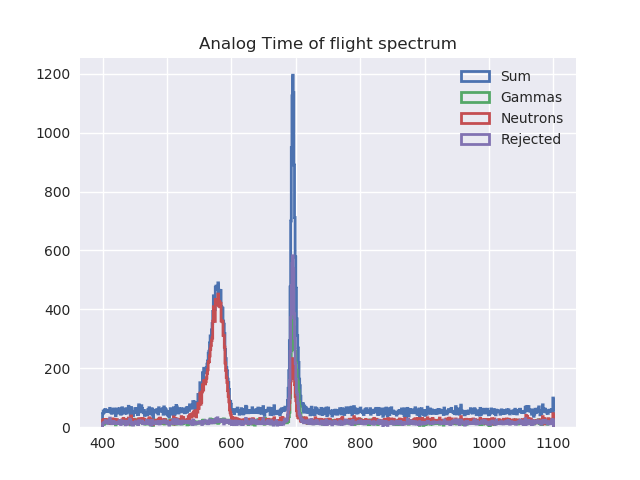
\includegraphics{AnalogResults/tof_psd.pdf}
        \caption[Heat map of pulse shape as a function of time of flight.]{Time of flight plotted against pulse shape as recorded with the analog setup. The dashed white line indicates the discrimination cut at PS=0.259. A logarithmic z-axis is used to highlight the distribution of background events.}
    \label{fig:tof_ps_a} 
\end{figure}


Often the start and stop signal will be due to uncorrelated particles, rather than the previously discussed n-\textgamma and \textgamma-\textgamma pairs. On small timescales of a few hundred nanoseconds these events are expected to form a flat background in the time of flight spectrum, as seen in figure \ref{fig:tof_a} beyond 60 ns. Since the events still represent either neutrons or gamma rays (ignoring the occasional muon) one would expect them to be separated into two bands in figure \ref{fig:tof_ps_a}. This is not the case.

Another interesting feature is that there is large amount of gamma rays at higher PS values. This is because not all the events produced by the pedestal injection were removed by the cut at 0.8 $\text{MeV}_\text{ee}$ and as these events use the same signal as start and stop, they will appear near the gamma peak. The reason why they have such a high fraction of PS lies in the gate lengths. Since the charge integrals of these events are just integrals of what randomly happened to be in the detector at the time a YAP trigger occurred, and since the longgate window is more than eight time as long as the shortgate window it is more likely that there is something to integrate in the tail part of the window.



\section{Digital setup}

\subsection{Neutron Tagging}
The time of flight spectrum acquired with the digital setup is shown in figure \ref{fig:tof_d}, with the gamma ray and neutron peaks indicated by arrows. The gamma peak is not entirely narrow as one might expect seeing as they all travel at the speed of light. The main reason for this is the intrinsic time resolution of the detector as well as the digitization of the pulse. The CFD algorithm looks for where the pulse crosses 30\% of maximum amplitude, but the determination of the maximum amplitude is limited by the resolution and sampling rate of the digitizer.

\begin{figure}[ht]
    \centering
        \includegraphics{DigitalResults/tof.pdf}
        \caption[Time of flight spectrum, digital setup.]{The time of flight spectrum of the PuBe source produced by the digital setup. The flight times in the red shaded region has been used to calculate the energy spectrum shown in the upper right insert.}
    \label{fig:tof_d} 
\end{figure}

The flight times in the neutron peak, shaded red, have been used to generate the energy spectrum shown in the upper right insert of figure \ref{fig:tof_d}. The same time and energy range used for the analog setup has been used here (29-\SI{62}{\ns} and 1.5-\SI{7}{\MeV} respectively). 

The spectrum goes to lower energies than what we see for the analog setup in figure \ref{fig:tof_a}, this may be because the digital setup has a lower amplitude threshold than the analog setup, allowing slower neutrons, which tend to deposit less energy in the detector, to be recorded.

Comparing with the reference spectrum shown in figure \ref{fig:scherzinger} the  \SI{3}{MeV} peak is apparent in both spectra. The small peak seen at \SI{4.8}{MeV} in the reference spectrum is however not present here. Since neutron pulses generally are well below 400 mV amplitude this can not be related to the limited available dynamic range.

\subsection{Pulse shape discrimination}
Just like with the analog setup \SI{500}{ns} and \SI{60}{ns} charge integrals were used to perform pulse shape discrimination. The parameters a and b in equation \ref{eq:ps} were chosen in order to linearize the separation between the bands. In the digital setup, where each pulse is digitized, these offsets can be interpreted as voltage offsets of the sampling points. During shortgate integration each sample point was offset by 4.79 mV while during longgate integration each sample point was offset by 0.24 mV .

The resulting PSD heat map is shown figure \ref{fig:psd_d}. The \SI{2.23}{\MeV} amd \SI{4.44}{MeV} Compton edges are indicated with arrows in the gamma ray band. The gamma ray band also contains a large concentration of low energy gamma rays near the threshold, which was not apparent in the analog PSD spectrum, due to a higher threshold. This large concentration is located below \SI{1}{MeV}, so it is likely to be gamma rays produced by deexcitation of $\text{234}$U.
A cut at PS=0.222 separates the neutron and gamma bands, although the two distributions overlap at lower energies.

\begin{figure}[ht]
    \centering
        \includegraphics{DigitalResults/psd.pdf}
        \caption[PSD spectrum, digital setup.]{Pulse shape discrimination spectrum produced with the charge comparisson method.}
        \label{fig:psd_d}
\end{figure}

%\subsection{Convolutional Neural Network}
The convolutional neural network described in \ref{sec:cnn} was applied to the digitized waveforms. The network was trained to ascribe a value between 0 and 1 depending on how much a signal looks like a neutron or a gamma ray. The result is shown in figure \ref{fig:cnn_E} as a function of deposited energy. 

Like for the charge comparison method the upper distribution is neutrons and the lower distribution consists of gamma rays. The two bands are separated by a cut at prediction=0.5. In order to highlight that the distributions overlap slightly at lower energies the z-axis has been strongly suppressed. The low energy concentration associated with deexcitation of $\text{234}$U as well as the the two Compton edges are distinguishable, although the \SI{2.23}{\MeV} is less concentrated.

\begin{figure}[ht]
    \centering
        \includegraphics{DigitalResults/CNNpsd.pdf}
        \caption[PSD spectrum obtained with CNN]{Pulse shape discrimination spectrum produced with a convolutional neural network. The z-axis has been strongly suppressed in order to make it visible at which energies the network has trouble discriminating.}
    \label{fig:cnn_E} 
\end{figure}

In figure \ref{fig:tof_cc_tof_cnn} PS as well as CNN prediction are shown as functions of the time of flight. Logarithmic z-axes are used to highlight the background distributions. Figure \ref{fig:tof_digi_cc} shows the narrow gamma distribution and the wider neutron distribution as separated by the charge comparison method. It is apparent that the two distributions overlap somewhat in pulse shape. It is also of note that the neutron and gamma background forms two slightly separated bands.  In figure \ref{fig:tof_digi_cnn} it can be seen that the CNN method provides a better separation, although it still appears that gamma and neutron distributions overlap slightly near prediction value 0.5. The distribution of random coincidence events clearly separate into a gamma ray band below the cut and a neutron band above it.


\begin{figure}
    \centering
    \begin{subfigure}[ht]{\textwidth}
        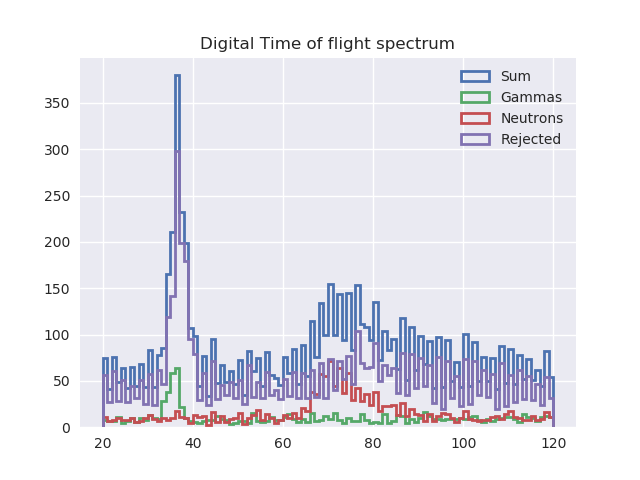
\includegraphics{DigitalResults/tof_psd.pdf}
        \caption{}
        \label{fig:tof_digi_cc}
    \end{subfigure}
	\begin{subfigure}[ht]{\textwidth}
        \includegraphics{DigitalResults/CNNtof_psd.pdf}
        \caption{}
        \label{fig:tof_digi_cnn}
    \end{subfigure}
    \caption[Pulse shape parameters as function of time of flight, digital setup.]{Heatmaps of of pulseshape discrimination parameters as functions of time of flight plotted with logarithmic z-axis.}
    \label{fig:tof_cc_tof_cnn}
\end{figure}

The heatmap shown in figure \ref{fig:tof_E_d} shows energy deposition in the NE213 detector as a function of time of flight. The gamma ray distribution is constituted of gamma rays that were produced in the deexcitation of $^\mathrm{12}$C or in deexcitation of $^\mathrm{234}$U as described in the chapter \ref{ch:1}. $^\mathrm{12}$C is primarily excited to the \SI{4.44}{\MeV} state. $^\mathrm{234}$U on the other hand can be excited to a wide range of states with excitation energies between \SI{13}{keV} and \SI{678}{keV}\cite{Nudat}.It is apparent that the low energy gamma rays are particularly dominating in the gamma ray time of flight peak.

The \SI{2.23}{MeV} gamma peak seen in the PSD and Energy spectra should not be visible in figure \ref{fig:tof_E_d} as these gamma rays are produced in an entirely different process by neutrons being absorbed by hydrogen nuclei. Strangely However, the figure shows a nearly continuous distribution of gamma rays from 0 up to around \SI{4.5}{MeV}.

\begin{figure}[ht]
    \centering
        \includegraphics{DigitalResults/tof_E.pdf}
        \caption[Time of flight plotted against energy deposition.]{Time of flight plotted against energy deposition.}
    \label{fig:tof_E_d} 
\end{figure}

The neutron distribution shows a relation between time of flight and deposited energy. The slowest neutrons have a smaller spread in deposited energy, whereas the faster ones have a much wider spread. This is because the neutron in each elastic scattering can loose up to a certain fraction of it's total kinetic energy, as described by equation \ref{eq:scat}. In NE213 the neutron primarily scatters against hydrogen nuclei. By equation \ref{eq:scat} it is then possible for the neutron to deposit anywhere between 0 and 100\% of its energy, with 0\% implying the neutron missed the nucleus and 100\% implying a head on collision.

In figure \ref{fig:N_E} this relation is highlighted. The top panel shows the ratio of deposited energy to neutron kinetic energy as a function of neutron energy. The red point represent the center of Gaussian functions fitted to the ratio of deposited to kinetic energy for narrow slices of neutron kinetic energies. the dotted line is the center point of the same type of fit covering all neutron energies. The ratio is nearly constant over the entire energy range, which suggests that the relation between deposited energy and neutron kinetic energy is approximately linear.

In fact the scintillation light output produced by an NE213 detector is expected to follow the following equation\cite{Scherzinger:2016}, Which approaches a linear shape at as neutron energies rise and the exponential term approaches unity:
\begin{equation}
	E_{deposited} = C\left(  0.83\cdot E_{neutron} - 2.82\cdot\left(  1 - e^{(-0.25\cdot E_{neutron}^{0.93})}  \right)  \right)
\end{equation}
The parameter C depends on the particular detector and can be found through fitting. In the bottom panel of figure \ref{fig:N_E} each red point represents the center of a Gaussian fitted to the deposited energies corresponding to a narrow slice of neutron energies. The value of C was found to be 0.794. The fact that the fit doesn't match the points so well at lower neutron energies may be due to the amplitude threshold particularly affects the low energy neutrons.

\begin{figure}[ht]
    \centering
        \includegraphics{DigitalResults/N_E.pdf}
        \caption[Neutron kinetic energy and deposited energy.]{Top: Ratio of deposited energy to neutron kinetic energy. Bottom: deposited energy as a function of neutron kinetic energy, along with fits.}
    \label{fig:N_E} 
\end{figure}

\section{Results and Performance Comparisson}\label{sec:comp}
\subsection{Energy Spectra and Livetime}
The analog and the digital setup were run with different amplitude thresholds, so in order to properly compare them the correct threshold need to be found. Since the two setups have different cable lengths to the detectors they are not attenuated to the same extent, so the digital setup will need a significantly higher threshold than the analog setup in order to accept the same events. Figure \ref{fig:qdc_comp} top panel shows the energy spectra from both setups.

The analog setup have been rescaled to compensate for the 56\% deadtime. The blue histogram shows the spectrum recorded with the digital setup, and the green histogram shows the same spectrum after applying a higher amplitude threshold of \SI{151}{mV} and normalizing the spectrum to match the height of the livetime corrected analog setup. This very crude estimation of the digital setups livetime gives a livetime of 12\% compared to the analog setups livetime of 44\%. By carrying out these changes the two energy spectra look more alike, although the \SI{4.44}{\MeV}$_\text{ee}$ Compton edges look quite different. This may be because some of the high energy gamma rays were outside of the dynamic range of the digitizer.

\begin{figure}[h]
    \centering
        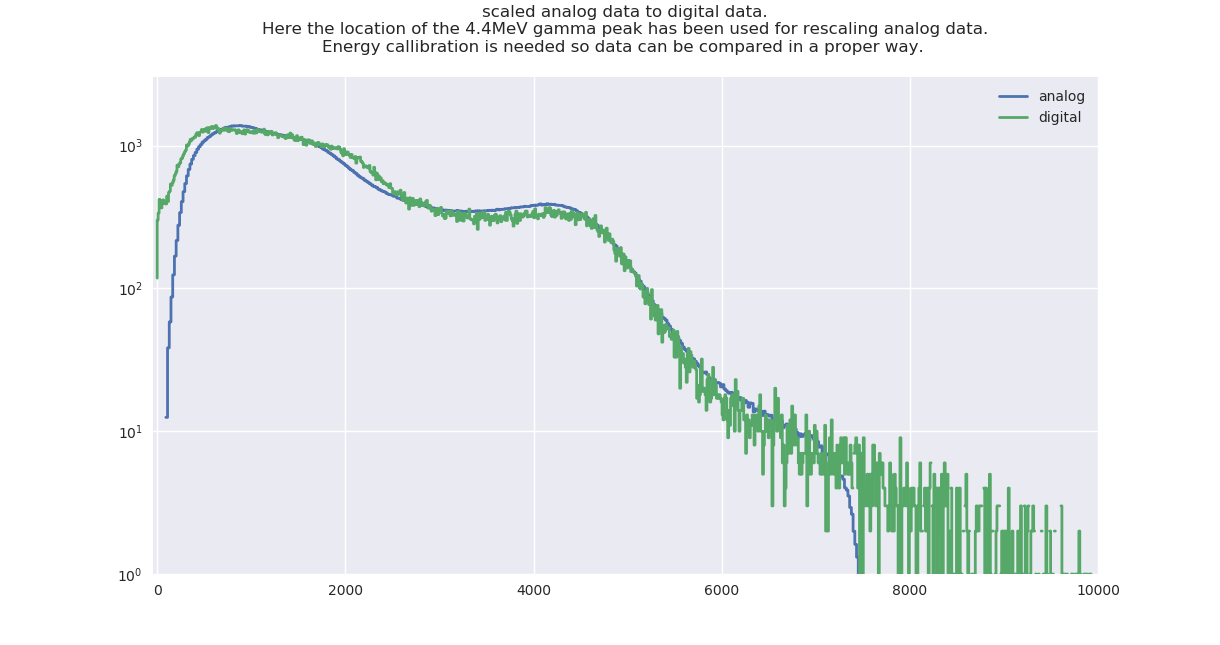
\includegraphics[width=0.8\textwidth]{CompareResults/qdc_comp.pdf}
        \caption[Comparison of analog and digital NE213 energy spectra]{Comparison of analog and digital NE213 energy spectra. The blue histogram is the raw digital energy spectrum and the red one has been normalized to the height of the analog spectrum, and has had a pulse height threshold of 151 mV applied.}
    \label{fig:qdc_comp}
\end{figure}

Figure \ref{fig:qdc_comp} bottom panel shows the ratio between the digital and analog Energy spectra from after livetime adjustments and threshold alignment. Below \SI{0.8}{\MeV}$_\text{ee}$ the analog setup will minimize the ration down due to the pedestal injection and above \SI{6}{\MeV}$_\text{ee}$ the ratio blows up because this is outside the range of the analog QDC modules. Ideally however everything in between 0.8 and \SI{6}{\MeV}$_\text{ee}$ should be very close to 1. Initially this seems to be the case, but near the \SI{4.44}{\MeV}$_\text{ee}$ Compton edge there is a bump followed by a valley. This is likely because the highest amplitude digitized pulses were clipped, causing them to be pushed to lower values of deposited energy.
%\begin{figure}[h]
%    \centering
%        \includegraphics[width=0.8\textwidth]{CompareResults/%QDC_ratio.pdf}
%        \caption{Ratio of the digital and analog energy spectra.}
%    \label{fig:qdc_ratio}
%\end{figure}

\subsection{Time of Flight Spectra}
Like the energy spectrum the time of flight spectrum is heavily influenced by the choice of amplitude threshold. Figure \ref{fig:tof_comp} top panel shows the time of flight spectra for the two setups with the initial 49 mV NE213 threshold on the digital setup and 94.6 mV on the analog setup. Interestingly it seems that the analog setup is cutting away the slower neutrons of this spectrum by setting a high amplitude threshold. By applying the new NE213 threshold of 151 mV to the digital setup and adjusting the livetime of both setups in the same manner as for the energy spectrum the time of flight spectrum shown in the bottom panel of figure \ref{fig:tof_comp} is obtained. There are more counts in the digitized time of flight spectrum. This is because the YAP thresholds have not been aligned. Secondly the neutron peaks now have roughly the same shape, which means that the amplitude cut has removed the slower neutrons. Additionally, with a full width at half maximum of the gamma peak of \SI{7.67}{\ns} the analog setup seems to have a poorer time resolution than the digital setup which has a FWHM of 2.75 ns at the gamma peak.

\begin{figure}[h]
    \centering
        \includegraphics[width=0.8\textwidth]{CompareResults/tof_comp.pdf}
        \caption[Comparison of analog and digital time of flight spectra.]{Comparison of analog and digital time of flight spectra. In the lower panel livetime has been taken into account and the digitized data has had a higher threshold enforced on the NE213 signals.}
    \label{fig:tof_comp}
\end{figure}

\subsection{PSD Performance}
By fitting Gaussian functions to the neutron and gamma distribution shown in \ref{fig:fom_analog} and \ref{fig:fom_digital} one can express the quality of separation between the two distribution as a figure of merit, F, defined in terms of the centers, C, of the Gaussian functions and their full width at half maximum, W. Thre greater F is the better.

\begin{equation}
F = \frac{C_n - C_\gamma}{W_n + W_\gamma}
\end{equation}

figure \ref{fig:fom_analog} and figure \ref{fig:fom_digital} shows histograms of the PS parameter along with the Gaussian fits used to calculate F. This way of parameterizing the quality of a PSD method requires that the distributions are approximately Gaussian. This assumption appears to be valid for the neutron distributions, centered at 0.3, but both figure \ref{fig:fom_analog} and figure \ref{fig:fom_digital} shows a tail on the gamma distributions which is not matching with the fit. The assumption of Gaussian distributions is not valid for the distributions produced by the CNN method, so the figure of merit, F, will only be used for comparing the charge comparison methods. 


\begin{figure}[h]
	\begin{subfigure}[b]{\textwidth}
	    \centering
    	    \includegraphics[width=0.65\textwidth]{CompareResults/FOM_analog.pdf}
        	\caption{Analog setup}
	    \label{fig:fom_analog} 
	\end{subfigure}
	\begin{subfigure}[b]{\textwidth}
    	\centering
        	\includegraphics[width=0.65\textwidth]{CompareResults/FOM_digital.pdf}
        	\caption{Digital setup}
    	\label{fig:fom_digital} 
    \end{subfigure}
    \caption[Histograms of pulseshape, with Gaussian fits.]{Histograms of pulseshape, with Gaussian fits to the gamma ray and neutron distributions. The inserts show the pulse shape parameter as a function of energy, for full size version see fig \ref{fig:psd_a} and \ref{fig:psd_d}. }
\end{figure}

Looking at the inserts in both figures it can be seen that F is highly energy dependent and that the digital setup outperforms the analog setup at at all energies. For details on this energy dependence see appendix \ref{ch:appA}. 

Another way to compare the performance of the PSD methods is by estimating the misclassification rate. This can be done by evaluating the time of flight spectrum in three different regions and comparing the relative number of neutron and gamma ray labeled events. Ideally the number of gamma rays identified per nanosecond channel in a background region, containing only random coincidences, should be the same as the number of gamma rays identified in the neighborhood of the neutron time of flight peak. Likewise the number of neutrons identified at the gamma peak should correspond to the neutron background. The misclassification rate of gamma rays and neutrons, 
M$_{\gamma}$ and M$_\textrm{n}$ respectively can be expressed as

\begin{equation}
	M_\gamma(R_\gamma) = \frac{N_{n}(R_\gamma)-\langle N_n(R_\gamma)\rangle}{N_{total}(R_\gamma)-\langle N_n(R_\gamma)\rangle}
\end{equation}

\begin{equation}
	M_n(R_n) = \frac{N_{\gamma}(R_n)-\langle N_\gamma(R_n)\rangle}{N_{total}(R_n)-\langle N_\gamma(R_n)\rangle}
\end{equation}
Where N$_n$ and N$_\gamma$ are the number of neutrons and gamma rays identified in region R and $\langle \textrm{N}_\textrm{n}\rangle$ and $\langle \textrm{N}_\gamma\rangle$ are the expected numbers found by normalizing the background rates to the width of R.

This definition of misclassificaton rate is relying on the assumption that the background is approximately flat and varies slightly with the choice of limits. However as long as the peaks were contained in the region the misclassification rates in percent were found to change by at most $\pm$2\%. The neutron peak limits were set to math the range of neutron energies 1.5-\SI{7}{\MeV} and the gamma peak neighborhood was selected as \SI{5}{\ns} on either side of the gamma ray peak.

Figure \ref{fig:tof_cc_cnn} shows the time of flight spectrum obtained with the analog setup filtered according to the charge comparison method, as well as the spectrum obtained from the digital setup, filtered by charge comparison and by the CNN. Gamma rays are colored blue, neutrons red and their intersection is purple. Ideally the intersection of the distributions should be flat, but if there is some systematic misclassification, then the intersection will rise up above the background level at the neutron and gamma peaks. This is an expression of the extent of misclassification of the given PSD implementation.

For the analog setup a high degree of contamination is evident in the form of the two purple peaks coinciding with the neutron and gamma peaks. This gives an estimated misclassification of 13\% for neutrons and 12\% for gamma rays. From figure \ref{fig:tof_ps_a} it was found that a number of the injected YAP start triggers remained even after cutting away events below \SI{0.8}{\MeV}, and that these landed at the gamma ToF but with very high PS values. These events may be part of the reason why there is nearly 12\% misclassification near the gamma ray peak.

The digital setup provides a lower misclassification rate with the charge comparison method, at 10\% for neutrons and 3\% for gamma rays. The much higher misclassification for neutrons imply that the model is biased towards gamma rays.

The CNN approach reaches even better results with gamma ray misclassification of 4\% and neutron misclassification rate of 5\%.
This is a significant improvement compared to the charge comparison method, and with the misclassification of nearly the same amount for both neutrons and gamma rays the CNN method does not appear to have a strong bias towards either particle species.

The neutron background is found to be nearly the same by the analog and digital charge comparison methods, at 37\% and 38\% respectively. The CNN method finds a significantly higher background of neutron events at 45\%. This together with the high misclassification rates for the charge comparison methods hints at them being biased towards gamma rays.

The correct fraction of events due to neutrons interacting in the NE213 is not trivial to determine. Although the radiation emitted by the source is approximately isotropic radiation scattered by the aquarium and walls of the room complicates matters. So to get a better idea of what fraction of neutrons to expect simulations are needed. It is however clear that the CNN distribution is better at reproducing a flat background of neutrons at the gamma peak and vice versa, than the digital and analog charge comparison methods, so it seems likely that 45\% is a better estimate.



\begin{figure}
    \centering
    \begin{subfigure}[bh]{\textwidth}
   	   	\centering
	    \includegraphics[\textwidth]{AnalogResults/ToF_filt.pdf}
    	\caption{Time of flight spectrum filtered by a linear cut at PS = 0.259.}
    	\label{fig:ToF_filt_A}
   	\end{subfigure}
    \begin{subfigure}[bh]{\textwidth}
   	    \centering
        \includegraphics[width=0.85\textwidth]{DigitalResults/ToF_filt.pdf}
        \caption{Time of flight spectrum filtered by a linear cut at PS=0.222.}
        \label{fig:ToF_filt_D}
    \end{subfigure}
	\begin{subfigure}[bh]{\textwidth}
	    \centering
        \includegraphics[width=0.85\textwidth]{DigitalResults/CNNToF_filt.pdf}
        \caption{Time of flight spectrum filtered by a linear cut at prediction = 0.5.}
        \label{fig:ToF_filt_D_CNN}
    \end{subfigure}
	\caption[Misclassification of different PSD implementations.]{Misclassification of different PSD implementations.}
    \label{fig:tof_cc_cnn}
\end{figure}






\end{document}